\documentclass[oneside,listof=totoc]{scrbook}
\setuptoc{toc}{totoc}
\linespread{1.5}
\usepackage{geometry}
\geometry{
  a4paper,
  lmargin=40mm,
  rmargin=30mm,
  tmargin=40mm,
  bmargin=30mm
}
\usepackage{fontspec}
  \setmainfont{Times New Roman}

\usepackage{pgf, tikz}
\usepackage{caption}

\usepackage[titles]{tocloft}
\setlength{\cftchapnumwidth}{38pt}
\renewcommand{\cftchappresnum}{\chaptername\ }
\renewcommand{\cftchapdotsep}{\cftdotsep}
\renewcommand{\cftchapfont}{\normalfont\bfseries}
\renewcommand{\contentsname}{Daftar Isi}
\renewcommand{\listfigurename}{Daftar Gambar}
\renewcommand{\listtablename}{Daftar Tabel}

\renewcommand{\chaptername}{BAB}
\renewcommand{\thechapter}{\Roman{chapter}}
\renewcommand{\thesection}{\thechapter.\arabic{section}}
\renewcommand{\thesection}{\arabic{chapter}.\arabic{section}}
\renewcommand{\thesubsection}{\arabic{chapter}.\arabic{section}.\arabic{subsection}}
\usepackage{titlesec}
\titleformat{\chapter}[display]
  {\Large\bfseries\centering}{\chaptertitlename\ \thechapter}{12pt}{}
  \titlespacing*{\chapter}{0pt}{-\topskip}{0pt}
\titleformat{\section}
  {\large\bfseries}{\thesection}{12pt}{}

\renewcommand{\figurename}{Gambar}
\renewcommand{\tablename}{Tabel}

\usepackage{fancyhdr}
\pagestyle{fancy}
\fancyhf{}
\fancyhead[R]{\thepage}
\renewcommand{\headrulewidth}{0pt}

\begin{document}

\frontmatter

\clearpage
\thispagestyle{empty}

\begin{center}
  \LARGE{\textbf{TUGAS}}\\
  \vspace{1.0cm}
  \Large{\textbf{JUDUL DITULIS SECARA SIMETRIS}}\\
  \Large{\textbf{PEMROGRAMAN VB.NET}}\\
\end{center}

\vspace{2.0cm}

\begin{minipage}{13cm}
  \centering
    
\includegraphics[width=6cm]{figures/vim_logo}
\end{minipage}

\vspace{1.5cm}

\begin{center}
  \normalsize{Disusun oleh:}\\
  \vspace{0.5cm}
  \begin{minipage}{\textwidth}
    \begin{center}
      \begin{tabular}{l r l }
        \textbf{Nama}  & : & \textbf{Rizqi Nur Assyaufi}\\
        \textbf{NIM}   & : & \textbf{20.02.222}
      \end{tabular}
    \end{center}
  \end{minipage}
\end{center}

\vspace{2.0cm}

\begin{center}
  \large{\textbf{PROGRAM STUDI TEXT EDITOR}}\\
  \large{\textbf{FAKULTAS VIM TEXT EDITOR }}\\
  \large{\textbf{UNIVERSITAS EDITOR}}\\
  \large{\textbf{BALIKPAPAN}}\\
  \large{\textbf{2020}}
\end{center}

\clearpage
\thispagestyle{empty}

\tableofcontents
\listoffigures
\listoftables

\mainmatter
\chapter{PENDAHULUAN}
\section{Sekilas Visual Basic.Net}
Visual Basic.Net (VB.Net) adalah salah satu bahasa pemrograman yang teradpat di dalam Visual Studio. VB.Net adalah bahasa pemrograman yang berorientasi dengan objek.Banyak software-software bisnis yang dibuat dengan bahasa pemrograman ini, karena lengkapnya toolbox yang bia digunakan untuk membuat software yang berkualitas. Gambar \ref{fig:awal_vb} berikut ini adalah tampilan dari VB.Net 2013.

\vspace{1.0cm}

\begin{minipage}{\linewidth}
  \centering
  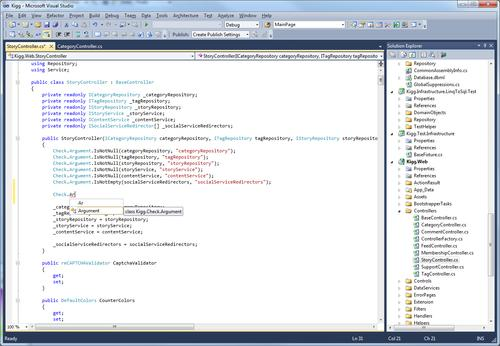
\includegraphics[width=10cm]{figures/fig_tampilan_awal_vb}
  \label{fig:awal_vb}
  \captionof{figure}{Tampilan antar muka VB.Net 2012}
\end{minipage}

\vspace{1.0cm}

Pada buku ini, VB.Net versi berapapun dapat kita gunakan, karena sintaks yang digunakan adalah sintaks yang juga sama pada berbagai versi dari VB.Net.

\section{Tipe Data}
Ada beberapa variabel yang terdapat dalam VB.Net, namun dalam buku ini hanya akan dibahas 3 jenis variabel yaitu integer, double dan string. Kita mulai dari integer, dalam bahasa Indonesia integer berarti bilangan bulat. Integer bukanlah tipe data yang sangat luas hingga tak terbatas, tapi memiliki interval jarak, yaitu -2.147.483.648 sampai 2.147.483.647. Tipe data double adalah tipe data pecahan, tapi dapat pula menampilkan angka bulat. Sedangkan tipe data string adalah tipe data yang beisi karakter. Ciri dari tipe data string adalah diapit dengan tanda petik dua (").

\section{Membuat Variabel}
Berikut ini, akan diberikan contoh mengenai bagaimana cara membuat variabel string, gambar \ref{fig:gui_membuat_string} berikut ini adalah rancangan antar muka yang akan kita susun.

\vspace{0.5cm}

\begin{minipage}{\linewidth}
  \centering
  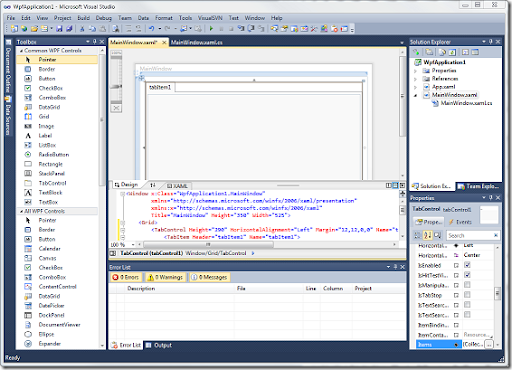
\includegraphics[width=10cm]{figures/fig_gui_membuat_form}
  \label{fig:gui_membuat_string}
  \captionof{figure}{Tampilan antar muka dari sebuah form}
\end{minipage}

\vspace{0.5cm}

Berikut ini adalah sintaks yang digunakan untuk membuat form.

\begin{verbatim}
Public Class Form1
  Private Sub Button1_Click(sender As Object, _
  e As EventArgs) Handles Button1.Click
    Dim tampil As String
    tampil = "Saya sedang belajar LaTeX"
    MsgBox(tampil)
  End Sub
End Class
\end{verbatim}

Blok kode di atas, diketik di dalam private sub Button1.Click, itu artinya sintaks di atas akan dieksekusi ketika button di klik. Dim tampil As String dalam blok kode di atas bermakna dimisalkan tampil adalah variabel dengan tipe data string, kemudian variabel string diisi dengan kalimat "Saya sedang belajar LaTeX". Variabel tampil yang sudah diisi, kemudian ditampilkan dalam message box.

Selanjutnya, kita kaan buat contoh yang kedua. Masih menggunakan antar muka yang sama, namun kali ini, namun kali ini kita akan memanggil variabel dengan tipe data integer.

\chapter{RUMUSAN MASALAH}
\section{Sekilas Visual Basic.Net}
Visual Basic.Net (VB.Net) adalah salah satu bahasa pemrograman yang teradpat di dalam Visual Studio. VB.Net adalah bahasa pemrograman yang berorientasi dengan objek.Banyak software-software bisnis yang dibuat dengan bahasa pemrograman ini, karena lengkapnya toolbox yang bia digunakan untuk membuat software yang berkualitas. Gambar \ref{fig:awal_vb} berikut ini adalah tampilan dari VB.Net 2013.

\end{document}
